\item La base de un sólido es el círculo $x^2 + y^2 = 7$. Hallar el volumen de dicho sólido si las secciones transversales perpendiculares al eje $x$ son
\begin{multicols}{2}
  \begin{enumerate}
    \item Cuadrados.
    \item Triángulos equiláteros.
  \end{enumerate}
\end{multicols} 

\item La base de un sólido es la región limitada por la elipse $4x^2 + 9y^2 = 36$. Hallar el volumen del sólido sabiendo que las secciones transversales perpendiculares al eje $x$ son
\begin{multicols}{2}
  \begin{enumerate}
    \item Triángulos equiláteros.
    \item Cuadrados.
  \end{enumerate}
\end{multicols} 

\item La base de un sólido es la región limitada por $y = x^2$ e $y = 4$. Hallar el volumen sabiendo que las secciones perpendiculares al eje $x$ son:
\begin{multicols}{2}
  \begin{enumerate}
    \item Cuadrados.
    \item Semicírculos.
    \item Triángulos equiláteros.
  \end{enumerate}
\end{multicols} 

\item La base de un sólido es la región comprendida entre las parábolas $x = y^2$ y $x = 3 - 2y^2$. Hallar el volumen del sólido sabiendo que las secciones perpendiculares al eje $x$ son 
\begin{multicols}{2}
  \begin{enumerate}
    \item Rectángulos de altura $h$.
    \item Triángulos equiláteros.
    \item Triángulos rectángulos isósceles, cada uno con la hipotenusa sobre el plano $xy$
  \end{enumerate}
\end{multicols} 

\item Hallar la fórmula para el volumen de un cono truncado en
función de su altura $h$, el radio de la base inferior $R$ y el radio de
la base superior $r$.

\centerline{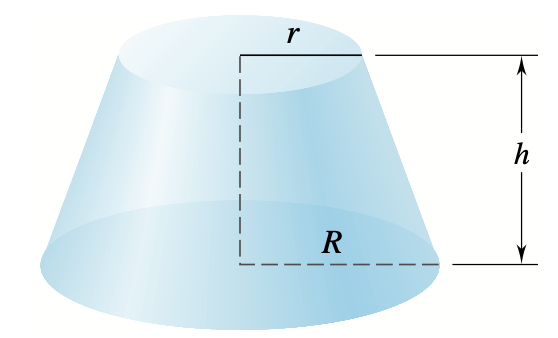
\includegraphics[width=.3\textwidth]{pics/cono-truncado.png}}

\item Un plano corta una esfera de radio $r$ a una altura de $h$ unidades
por encima del ecuador ($0 < h < r$). La parte superior de la
esfera se llama casquete. Deducir la fórmula de su volumen.

\item  La región que se muestra en la figura se rota alrededor de eje $y$
para formar un recipiente de forma parabólica. La unidades
indicadas están en metros. ?`Cuál es el volumen del recipiente?

\centerline{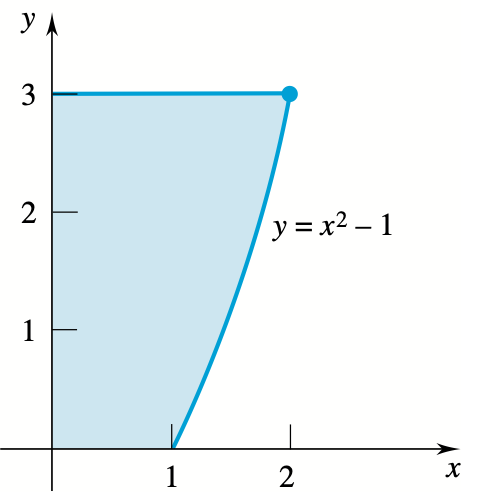
\includegraphics[width=.3\textwidth]{pics/recipiente-parabolico.png}}

